% !TeX program = pdflatex
\documentclass[tikz,border=8pt]{standalone}
\usepackage{tikz}
\usetikzlibrary{angles,quotes,positioning}
\definecolor{FigureBlue}{HTML}{2563EB}
\definecolor{FigureOrange}{HTML}{EA580C}
\definecolor{FigureSlate}{HTML}{64748B}
\begin{document}
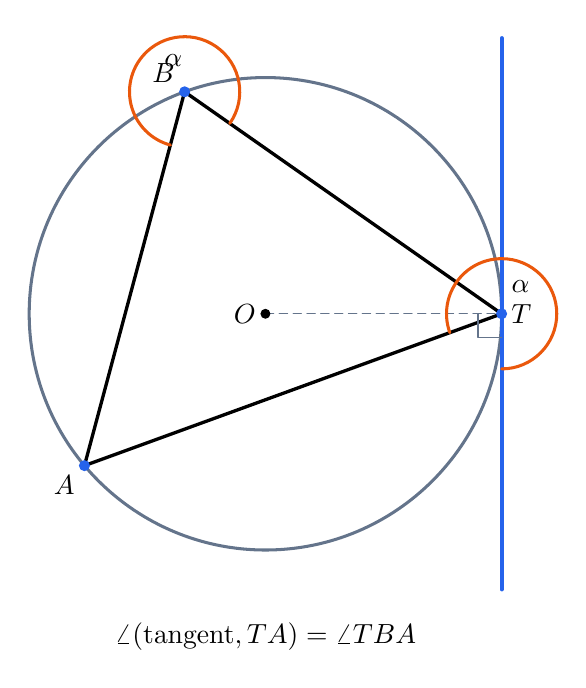
\begin{tikzpicture}[line cap=round,line join=round]
  \coordinate (O) at (0,0);\coordinate (T) at (3,0);\coordinate (S) at (3,-3);
  \coordinate (A) at (220:3);\coordinate (B) at (110:3);
  \draw[FigureSlate,line width=1.1pt] (O) circle[radius=3];
  \draw[FigureBlue,line width=1.5pt] (3,-3.5)--(3,3.5);
  \draw[line width=1.2pt] (T)--(A)--(B)--(T);
  \draw[FigureSlate,densely dashed] (O)--(T);
  \pic[draw=FigureOrange,line width=1.1pt,angle radius=7mm,"$\alpha$"] {angle=S--T--A};
  \pic[draw=FigureOrange,line width=1.1pt,angle radius=7mm,"$\alpha$"] {angle=T--B--A};
  \draw[FigureSlate] (2.7,0)--(2.7,-.3)--(3,-.3);
  \foreach \P in {T,A,B}{\fill[FigureBlue] (\P) circle (2pt);}\fill (O) circle (1.8pt);
  \node[left] at (O) {$O$};\node[right] at (T) {$T$};\node[below left] at (A) {$A$};\node[above left] at (B) {$B$};
  \node[below=8mm] at (0,-3) {$\angle(\hbox{tangent},TA)=\angle TBA$};
\end{tikzpicture}
\end{document}
